\documentclass{beamer}
\usetheme{Boadilla}
\usepackage{default}
\usepackage{graphicx}
\graphicspath{ {./images/} }

% fix footer
\makeatother
\setbeamertemplate{footline}
{
	\leavevmode%
	\hbox{%
		\begin{beamercolorbox}[wd=.4\paperwidth,ht=2.25ex,dp=1ex,center]{author in head/foot}%
			\usebeamerfont{author in head/foot}\insertshortauthor
		\end{beamercolorbox}%
		\begin{beamercolorbox}[wd=.6\paperwidth,ht=2.25ex,dp=1ex,center]{title in head/foot}%
			%\usebeamerfont{title in head/foot}\insertshorttitle\hspace*{3em}
			\insertframenumber{} / \inserttotalframenumber\hspace*{1ex}
		\end{beamercolorbox}}%
		\vskip0pt%
	}
	\makeatletter
	\setbeamertemplate{navigation symbols}{}

% add section frames
\AtBeginSection[]{
	\begin{frame}
		\vfill
		\centering
		\begin{beamercolorbox}[sep=8pt,center,shadow=true,rounded=true]{title}
			\usebeamerfont{title}\insertsectionhead\par%
		\end{beamercolorbox}
		\vfill
	\end{frame}
}

\title{Thumbs Up? Sentiment Classification using Machine Learning Techniques}
\subtitle{Pang, Lee, Vaithyanathan - EMNLP 2002}
\author{Slides by: Dor Cohen, Itai Gat}
\institute{IE\&M @ Technion}
\date{\today}

\newtheorem{snt}{Review example}
\begin{document}

% start
\begin{frame}
	\titlepage
\end{frame}

% commented
% agenda

\iffalse
\begin{frame}
	\frametitle{Agenda}
	\tableofcontents
\end{frame}
\fi

% intro
\section{Problem definition}

% intro pages - currently commented out
% motivation plays as intro instead


\begin{frame}
	\frametitle{Topic classification}
	\centering
	
\includegraphics[scale=0.4]{word_cloud}
\end{frame}

\iffalse
\subsection{Topic classification}

\begin{frame}
	\frametitle{Topic classification}
	\begin{itemize}
	\item Recent (2002) works sort documents according to their \textbf{subject}
	\begin{itemize}
		\item e.g., sports vs. politics
	\end{itemize}
	\pause
	\item Yet crucial part of online posted articles is their \textbf{sentiment}
	\begin{itemize}
		\item provide useful insights for readers automatically
		\item e.g., product review is negative or positive
	\end{itemize}

	\end{itemize}
\end{frame}

% commented
\iffalse
\begin{frame}
	\frametitle{Topic classification}
	\framesubtitle{Current (2002) techniques for non-topic text categorization}
	\begin{itemize}
		\item Source style with features as stylistic variation (Biber, 1988)
		\begin{itemize}
			\item e.g., author, publisher (NY times vs. Daily News)
		\end{itemize}
		\item Genre of text (Finn et al., 2002)
		\begin{itemize}
			\item e.g., editorial 'subjective' genre
		\end{itemize}
		\item Is subjective language used? (Wiebe et al., 2001)
		\item Does text contains opinion expressing?
	\end{itemize}
\end{frame}
\fi

\subsection{Sentiment analysis}

\begin{frame}
	\frametitle{Sentiment analysis}
	\begin{itemize}
	\item This work: apply topic classification techniques on sentiment analysis
	\begin{itemize}
		\item Q: What are our expected challenges?
		\pause %1
		\item A: Topics are identifiable by key words alone \\ detecting sentiment requires more \textbf{understanding}
	\end{itemize}
	\end{itemize}
	
	\pause %2
	\begin{itemize}
		\item e.g., "How could anyone sit through this movie?"
		\begin{itemize}
			\item Can you mark  any negative word?
		\end{itemize}
	
	\end{itemize}
	
	%\pause
	
	% other works
	%\begin{itemize}
	%\item Previous (2002) techniques:
	%\begin{itemize}
	%	\item Cognitive linguistic models (Sack, 1994)
	%	\item Discriminant word lexicons (Tong, 2001)
	%	\item Semantic orientation of words (Turney and Littman, 2002)
	%\end{itemize}
	%\end{itemize}

\end{frame}
\fi

\begin{frame}
	\frametitle{Sentiment analysis}
	\framesubtitle{Motivation}
	\begin{center}
	\begin{tabular}{c}
		
\includegraphics[scale=0.5]{imdb_star} \\
	\end{tabular}
	\end{center}
	\begin{itemize}
		\item Should we watch this movie? \pause
		\item Ideally: read each review and decide
	\end{itemize}
	\begin{center}
	\begin{tabular}{l}
		
\includegraphics[scale=0.5]{imdb_review_pos_exag} \pause \\ \hline \hline
		
\includegraphics[scale=0.5]{imdb_review_neg}
	\end{tabular}
	\end{center}

\end{frame}

% problem
\subsection{Problem definition}
\begin{frame}
	\frametitle{Problem definition}
	\begin{itemize}
		\item Find mapping from text to binary label
		\begin{itemize}
			\item Supervised learning
		\end{itemize} \pause
		\item For $m$ numeric features (extracted from text) we define:
	\end{itemize}
	\begin{definition}[Binary classifier]
		\center
		$f: X \to y$ \\
		where $X \in \mathbb{R}^{m}$, $y \in \{0,1\}$
	\end{definition}
	\pause
	\begin{itemize}
		\item Evaluate by loss function
		\item e.g., Zero-one loss: $L(x,y,f_w)=\textbf{1}\{ f_w(x) \neq y \}$
		\begin{itemize}
			\item $w$ denotes learned parameters
		\end{itemize}
	\end{itemize}
\end{frame}

\subsection{Data}

\begin{frame}
	\frametitle{Data: IMDB Movie Reviews}
	\begin{itemize}
		\item User rating provides \textbf{supervised} learning:
		%\item Converted into 3 categories:
		%\begin{itemize}
		%	\item \emph{Positive}, \emph{negative}, (\emph{neutral} - not used)
		%\end{itemize}
		%\item Avoid bias issues:
		%\begin{itemize}
		%	\item 20 reviews per author per sentiment
		%	\item 752 negative vs 1301 positive
		%	\item total of 144 reviewers
		%\end{itemize}
	\end{itemize}
	\begin{center}
		
\includegraphics[scale=0.4]{rating_bar}
	\end{center}
	\begin{center}
		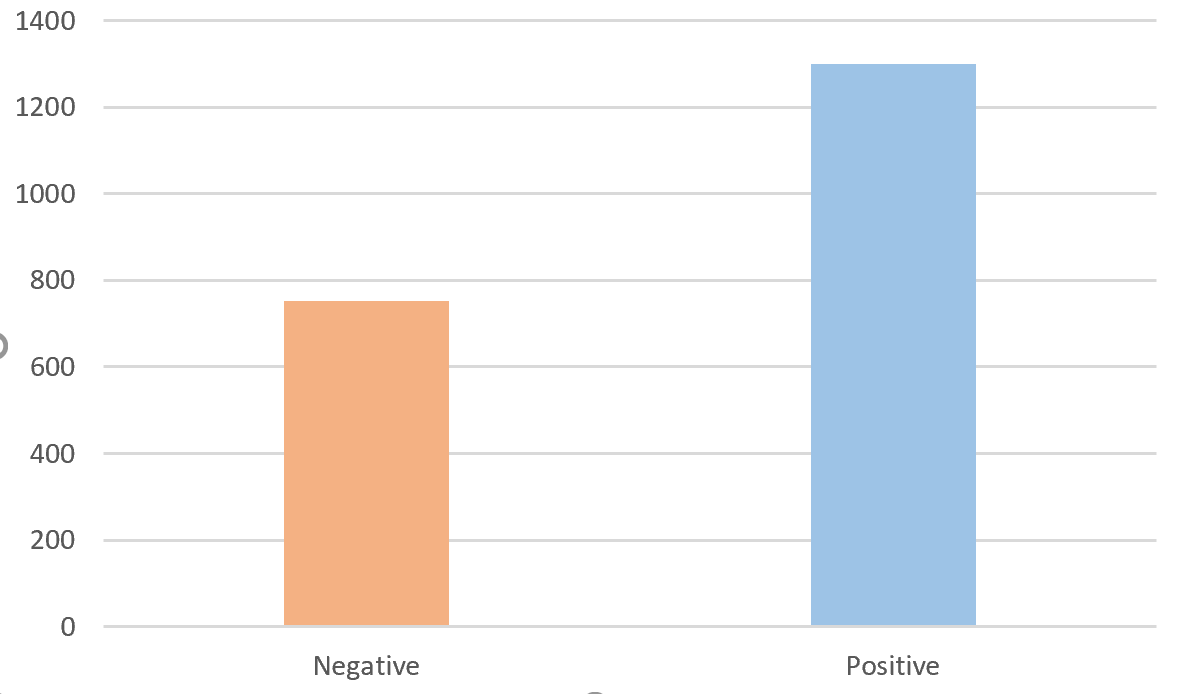
\includegraphics[scale=0.5]{reviews}
	\end{center}
\end{frame}

% human based

\subsection{Human baseline}
\begin{frame}
	\frametitle{Human based sentiment classifiers}
	\begin{itemize}
		%\onslide<1->
		%\item In contrast to topics, detecting sentiment is easier for us (why?)
		%\begin{itemize}
		
		%\onslide<2->
		%\item People tend to express strong feelings, topics can be related
		%\item Topics can be related, while with opinions people tend to express strong feelings
		%\end{itemize}
		
		%\onslide<3->
		\item \textbf{Hypothesis:} certain words indicate on sentiment type
		
		\item \textbf{Test:} count positive vs. negative words
	\end{itemize}
	
	%\onslide<5->
	\begin{table}
		\scriptsize
		\begin{tabular}{ l | p{5cm} | c | c }
			Human & Proposed words & Accuracy & Ties \footnotemark \\ \hline \hline
			1 & positive (5): dazzling, brilliant.. \newline negative (5): suck, terrible.. & 58\% & 75\% \\ \hline
			2 & positive (11): gripping, spectacular.. \newline negative (6): cliched, boring.. & 64\% & 39\%  \\  \hline
		\end{tabular}
		\caption{Baseline results for human word lists, data is balanced (700 vs. 700)}
	\end{table}
	
	 %\only<5->{\footnotetext{Documents percentage where sentiments rated equally}}
	 \footnotetext{Documents percentage where sentiments rated equally}
\end{frame}

\begin{frame}
	\frametitle{Human based sentiment classifiers}
	\framesubtitle{Should we worry about high rate of ties?}
	\begin{itemize}
		\item Proposed list is relatively short (usually effect is 0 vs. 0)
		\begin{itemize}
			\item Not necessarily the reason for low accuracy!
		\end{itemize}
		\item Authors propose their list
		\begin{itemize}
			\item Backed up with statistics
		\end{itemize}
	\end{itemize}
	
	\begin{table}
		\scriptsize
		\begin{tabular}{ l | p{5cm} | c | c }
			Human & Proposed words & Accuracy & Ties \\ \hline \hline
			3+Stats & positive (7): love, wonderful.. \newline negative (7): bad, worst, '?', '!',.. & 69\% & 16\% \\ \hline
		\end{tabular}
		\caption{Results where words (total 14) were chosen based on data statistics}
	\end{table}
	
\end{frame}

\begin{frame}
	\frametitle{Human based sentiment classifiers}
	\framesubtitle{(2018) Data analysis}
	We reproduced the analysis, following are example estimates
	\begin{center}
		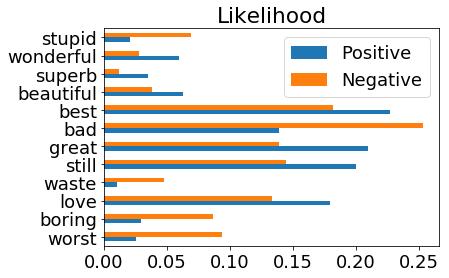
\includegraphics[scale=0.5]{likelihoods}
	\end{center}
	\begin{itemize}
		\item Note words occurrences were binarized
	\end{itemize}
\end{frame}

\section{Methods}
\subsection{Bag of words}

\iffalse
\begin{frame}
\frametitle{Bag of words}
\framesubtitle{Framework details}

\begin{theorem}[1]
	Let $\{f_1,..f_m\}$ denote set of m features that can appear in document.
\end{theorem}
\pause

\begin{itemize}	
	% introduce unigrams, bigrams
	% relative frequency, tf-idf
	\item $d$: "Audio quality rocks"
	\pause
	\item Features:
	\begin{itemize}
		\item Unigram: \{'audio', 'rocks',..  \}
		\item Bigram: \{'audio quality',.. \}
		\item N-gram !
	\end{itemize}
\end{itemize}

\pause
\begin{theorem}[2]
	Let $n_i(d)$ be the number of times $f_i$ occurs in document $d$.
\end{theorem}

\pause
\begin{Definition}[BOW]
	Then each document $d$ is represented by $d^{bow}:=(n_1(d),...,n_m(d))$.
\end{Definition}

\end{frame}
\fi

\begin{frame}
	\frametitle{Bag of words}
	\framesubtitle{Example}
	\begin{itemize}
		\item $d_1$: "Great soundtrack, boring actors"
		\item $d_2$: "Annoying soundtrack, great actors"
	\end{itemize}
	\begin{center}
	\begin{table}
		\begin{tabular}{c|c|c|c|c|c}
			& actors & soundtrack & boring & annoying & great \\ \hline \hline
			d1 & 1 & 1 & 1 & 0 & 1 \\
			d2 & 1 & 1 & 0 & 1 & 1
		\end{tabular}
	\end{table}
	\end{center}
	
	\begin{itemize}
		\item $d_3$: "Great soundtrack, great actors, great popcorn."
		\item $d_3^{bow}=$? \pause
		\item $d_3^{bow}$=(1,1,0,0,3)
	\end{itemize}
\end{frame}

\subsection{Naive bayes}
\begin{frame}
	\frametitle{Naive Bayes classifier}
	\begin{itemize}
		\item Assign class which maximizes: $c^{*}=argmax_{c} P(c|d)$
		\pause
		\item Recap:
	\end{itemize}
	
	\begin{Definition}[Bayes theorem]
		\center
		$P(c|d) = \frac{P(c)P(d|c)}{P(d)}$
	\end{Definition}
	\pause
	\begin{itemize}
		\item To estimate $P(d|c)$ we \textbf{naively} assume $f_i$'s are independent
		\pause
		\begin{itemize}
			\item Hence $\widehat{P(d|c)}=\prod_{i=1}^{m}P(f_i|c)^{n_i(d)}$ 
		\end{itemize}
		%\pause
		%\item Q: Any numeric issues you notice?
		%\pause
		%\item $A_1$: Estimates could be zero
		%\pause
		%\item $A_2$: Short vs. long documents
	\end{itemize}
\end{frame}

\begin{frame}
	\frametitle{Naive bayes example}
	Assume the following Bow model with 4 documents for each class:
	\begin{center}
		\begin{table}
			\begin{tabular}{c|c|c|c|c}
				& act & audio & boring & rocks \\ \hline \hline
				positive & 1 & 3 & 1 & 3 \\
				negative & 3 & 1 & 3 & 1
			\end{tabular}
		\end{table}
	\end{center}
	\pause
	\begin{itemize}
		\item $d_3$ = "Boring effects" , $d_3^{bow}=(0,0,1,0)$ \pause
		\item Recall $\widehat{P(d|c)}=\prod_{i=1}^{m}P(f_i|c)^{n_i(d)}$ \pause
		\item $P(d|pos)=\frac{1}{4}^0*\frac{3}{4}^0*\frac{1}{4}^1*\frac{3}{4}^0=\frac{1}{4}$ \pause
		\item $P(d|neg)=\frac{3}{4}^0*\frac{1}{4}^0*\frac{3}{4}^1*\frac{1}{4}^0=\frac{3}{4}$
	\end{itemize}
\end{frame}

\subsection{SVM, Logistic Regression}
\begin{frame}
	\frametitle{SVM vs. Logistic regression}
	\begin{itemize}
		\item Can view both parametrically: $ f(x_i,W) = Wx_i + b $
		\item \textbf{Train} with gradient descent:
		\begin{itemize}
			\item Initialize parameters
			\item 1. Update parameters following loss gradient
			\item 2. Repeat until convergence
		\end{itemize}
	\end{itemize}
	\pause
	Methods differ in their loss functions:
	\begin{definition}[SVM loss]
		$ L_i = \sum_{j \neq i}max(0, s_{j} - s_{y_{i}} + \delta)$, where $s_j = f(x_i,W)_j$
	\end{definition}
	
	\begin{definition}[Softmax loss]
		$ L_i = -log( \frac{ e^{f_{y_{i}}}  }{ \sum_{j} e^{f_{j}} }  ) $
	\end{definition}

\end{frame}

\begin{frame}
	\frametitle{SVM vs. Logistic regression}
	\framesubtitle{Evaluate loss example}
	\begin{center}
		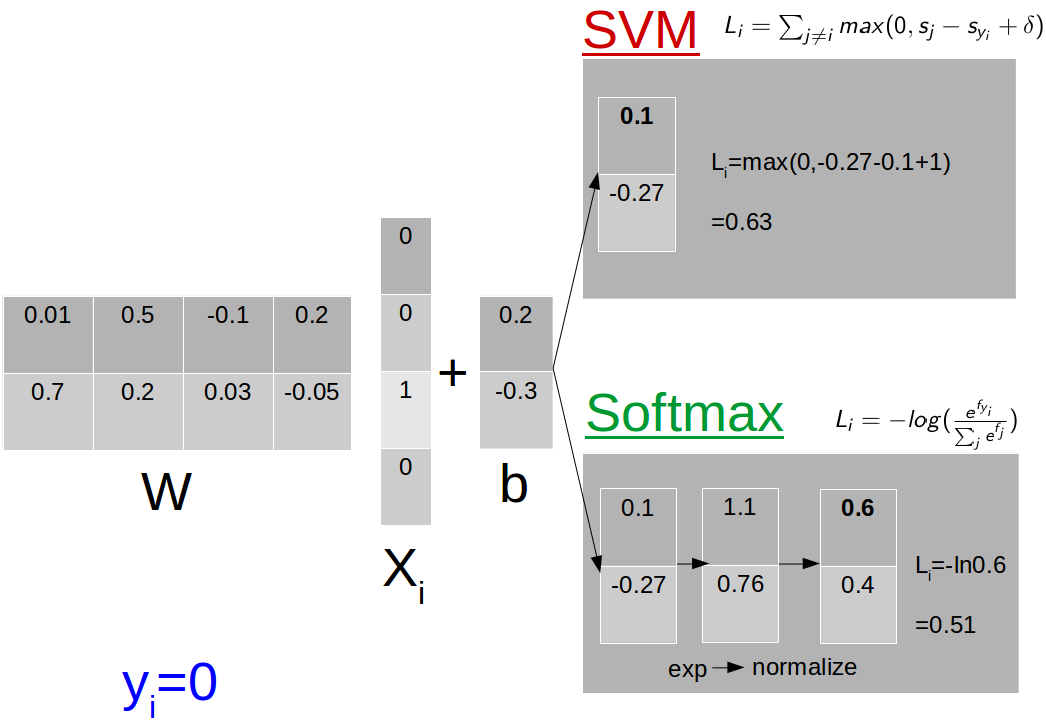
\includegraphics[scale=0.27]{svm_softmax_img}
	\end{center}
	
\end{frame}

\iffalse
\begin{frame}
	\frametitle{Logistic regression vs. SVM}
	\framesubtitle{Parametric view}
	\begin{definition}[Score function]
		$ f(x_i,W) = Wx_i + b $
	\end{definition}
	
	% something is wrong
	\begin{definition}[SVM loss]
		$ L_i = \sum_{j \neq i}(0,s_j-s_y_i + \delta)$
	\end{definition}
	
	\begin{definition}[Softmax loss]
		$ L_i = -log(\frac{e^f_y_i}{\sum_{j}e^f_j})$
	\end{definition}

	\begin{definition}[Gradient descent]
		\centering
		$w = w - \alpha * \frac{\partial L(X,w)}{\partial w} $ , Update till convergence
	\end{definition}

\end{frame}


\begin{frame}
	\frametitle{Maximum entropy classifier}
	\framesubtitle{aka logistic regression}
	\begin{Definition}[MaxEnt estimator]
		$P(c|d) = \frac{1}{Z(d)} exp(\sum_{i}\lambda_{i,c}F_{i,c}(d,c))$
	\end{Definition}
	\begin{itemize}
		\pause
		\item $Z(d)$ - normalization function
		\pause
		\item $F_{i,c}$ is a \emph{feature/class function}\
		\pause
		\begin{itemize}
			\item Defined: $F_{i,c}(d,c') = 1$ if feature $i$ \textbf{appears} on document $d$ and its estimated class is c, o.w. $F_{i,c}(d,c) = 0$
		\end{itemize}
		\pause
		\item $\lambda_{i,c}$ - feature-weight parameters 
		\begin{itemize}
			\item large values imply $f_i$ is a strong indicator for class c
		\end{itemize}

	\end{itemize}
	
	\pause
	\underline{Fit procedure}
	\begin{itemize}
		\item Training data used to estimate distribution $F$
		\item $\lambda$'s are set to maximize entropy of induced distribution
	\end{itemize}
			
\end{frame}

\subsection{SVM}
\begin{frame}
	\frametitle{Support vector machines}
	\begin{itemize}
		\item Goal: Find hyperplane $w$ which separates classes with margin large as possible \pause
		\item In this setting we define $w$ as:
	\end{itemize}
	
	\begin{Definition}[SVM hyperplane]
		Let $c_j \in \{1,-1\}$ be the class of document $d_j$ then: \\
		\centering{
		$w:=\sum_{j}\alpha_{j}c_{j}\overrightarrow{d_{j}}$, $\alpha_{j} \geq 0$} \\
	\end{Definition}
	\begin{itemize}
		\item $\alpha_{j}$ are obtained by solving dual optimization problem.
	\end{itemize}
	\pause
	\underline{Alternative fitting procedure:}
	\\
	\begin{Definition}[Gradient descent]
		\centering
		$w = w - \alpha * \frac{\partial L(X,w)}{\partial w} $ , Update till convergence
	\end{Definition}

\end{frame}
\fi

\section{Results}
\subsection{Experimental setup}
\begin{frame}
	\frametitle{Experimental setup}
\textbf{Features:}
\begin{itemize}	
	% introduce unigrams, bigrams
	%\item Experimented with various settings
	\item $d$: "Audio quality rocks"
	\item Unigram: \{'audio', 'rocks',..  \}
	\item Bigram: \{'audio quality',.. \}
	\item N-gram !
\end{itemize}

\textbf{Setup}
\begin{itemize}
	\item Unigram/bigram appear at least 4/7 times
	\item Uniform class distributions
	\item 3-fold average accuracies
	\item Unified NOT tag
%	\item Punctuation treated as separate lexicon, no stemming used
\end{itemize}
\end{frame}

\subsection{Results}

\iffalse
\begin{frame}
	\frametitle{Results and discussion}
	\begin{center}
		\begin{table}
			\begin{tabular}{l | l | l | l || l | l | l}
				ID & Features & count & freq/pres & NB & ME & SVM \\ \hline \hline
				1 & unigrams & 16165 & freq & 78.7\% & NA & 72.8\% \\
				2 & unigrams & 16165 & pres & 81.0\% & 80.4\% & \textbf{82.9}\% \\
			\end{tabular}
			\caption{3-fold average accuracies, unigrams appear at least 4 times on corpus.}
		\end{table}
	\end{center}
	\pause
	\begin{itemize}
		\item Recall human baseline ranges between $50\%-69\%$ \pause
		\item Topic-based classification reached $90\%+$ accuracy \pause
		\begin{itemize}
			\item Settings were multi-class
			\item We conclude that sentiment analysis is harder
		\end{itemize} \pause
		\item The frequency vs. presence of features seems to make the difference \pause
		\begin{itemize}
			\item Hence from this point authors use presence (\textbf{binarized occurrences})
		\end{itemize}
	\end{itemize}
\end{frame}
\fi

\begin{frame}
	\frametitle{Results and discussion}
	\framesubtitle{Using feature presence}
	\begin{center}
		\begin{table}
			\begin{tabular}{l | l | l || l | l | l}
				ID & Features & count & NB & ME & SVM \\ \hline \hline
				2 & unigrams & 16165 & 81.0\% & 80.4\% & \textbf{82.9}\% \\
				3 & uni+bigrams & 32330 & 80.6\% & 80.8 & \textbf{82.7}\% \\
				4 & bigrams & 16165 & 77.3\% & 77.4\% & 77.1\% \\ \hline \hline
				5 & unigrams+POS & 16695 & 81.5\% & 80.4\% & \textbf{81.9}\% \\
				6 & adjectives & 2633 & 77.0\% & 77.7\% & 75.1\% \\
				7 & top 2633 unigrams & 2633 & 80.3\% & 81.0\% & 81.4\% \\
				8 & unigram+position & 22430 & 81.0\% & 80.1\% & \textbf{81.6}\% \\
			\end{tabular}
			%\caption{3-fold average accuracies, unigram/bigrams appear at least 4/7 times on corpus. Expressions with negation words were handled with unified "NOT" tag. }
		\end{table}
	\end{center}
	\pause
	\begin{itemize}
		\item Adding bigrams doesn't improve results; Bigrams alone is worse
		\item Part-of-speech: "I love this movie" vs. "This is a love story"
		\item Position based on dividing text into quarters
	\end{itemize}
\end{frame}

\section{Conclusions}
\begin{frame}
	\frametitle{Conclusions}
	\begin{itemize}
		\item Unigrams presence setting achieves the best performance
		\begin{itemize}
			\item Apply feature selection algorithms
		\end{itemize}
		\item Contrarily, performance isn't comparable to topic classification 
	\end{itemize}
	
	\begin{snt}
		"This film should be brilliant. It sounds like a great plot, the actors are first grade, and the supporting cast is good as well, and Stallone is attempting to deliver a good performance. However, it can't hold up."
	\end{snt}
	\pause
	
	\begin{itemize}
		\item Difficult for bag-of-words classifiers
		\item Authors suggest determining the \textbf{focus} of each sentence
	\end{itemize}
\end{frame}

\iffalse
\section{Reproduce results}
\begin{frame}
	\frametitle{Reproduce results}
	\framesubtitle{(2018)}
	\begin{itemize}
		\item We have tried to reproduce the experiment for the best setting reported
	\end{itemize}
	\begin{center}
		\begin{table}
			\begin{tabular}{l | l | l || l | l | l}
				Features & count & NB & ME & SVM & MLP\\ \hline \hline
				unigrams & 16165 & 81.0\% & 80.4\% & \textbf{82.9}\% & NA \\
				unigrams & 16165 & 77.48\% & \textbf{81.52}\% & 80.66\% & \textbf{82.75}\%  \\
			\end{tabular}
			\caption{Original vs. our results}
		\end{table}
	\end{center}
	\begin{itemize}
		\item \textbf{No tuning} (sklearn 0.19.2 default parameters)
		\item MLP: 2-layer neural network, 100 Relu neurons, sigmoid
		\item Notebook is available \href{https://github.com/dorcoh/sentiment-emnlp/blob/master/experiment/sentiment-analysis-emnlp2002.ipynb}{\beamergotobutton{here}}
	\end{itemize}
\end{frame}

\begin{frame}
	\frametitle{Classifier comparison}
	\framesubtitle{(2018)}
	\begin{itemize}
		\item Our classifiers decision boundaries for some toy datasets
	\end{itemize}
	\begin{center}
		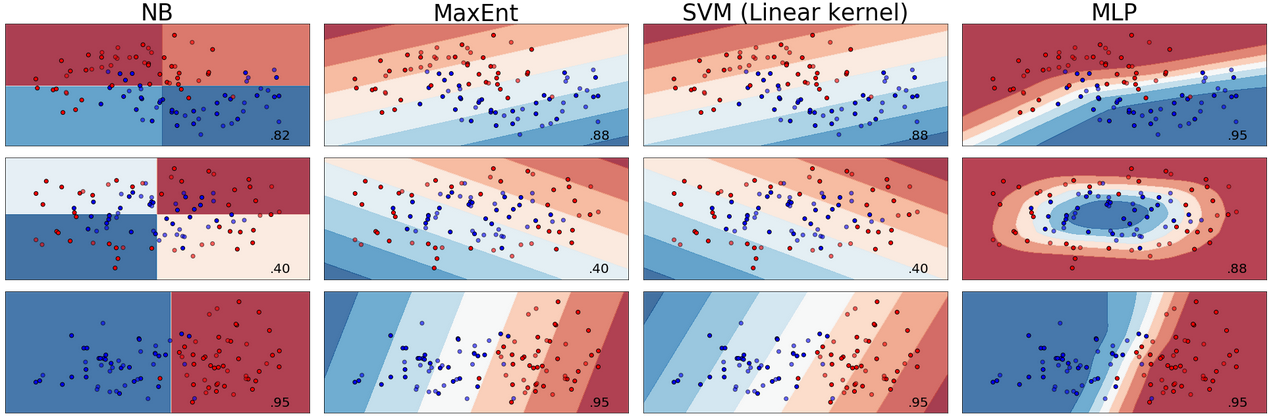
\includegraphics[scale=0.26]{comparison}
	\end{center}
	\begin{itemize}
		\item Accuracy is reported
	\end{itemize}
\end{frame}
\fi

\begin{frame}
	\centering
	\huge
	Thank you for participating! \\
	Questions?
\end{frame}

\end{document}
